\documentclass[11pt,a4paper]{article}
\usepackage[T1]{fontenc}
\usepackage[utf8]{inputenc}
\usepackage{lmodern,microtype}
\usepackage{amsmath,amssymb,amsthm,mathtools,bm}
\usepackage{booktabs,array,tabularx,longtable}
\usepackage{graphicx,float,caption}
\usepackage{xcolor}
\usepackage[margin=20mm]{geometry}
\usepackage{enumitem,fancyhdr}
\usepackage[hidelinks,unicode=true]{hyperref}
\hypersetup{
 pdftitle={FIN ST142--ST153: Natural Quotients, Constrained Selection, and Bath Resource Bounds},
 pdfauthor={Krzysztof Żuchowski},
 pdfsubject={Analytical and computational execution of FIN programs ST142--ST153},
 pdfkeywords={FIN, operator algebra, natural quotient, spectrahedron, Krawczyk, selector cost, symmetry breaking, causal net, hidden Markov model, thermal operation, minimax}
}
\setlength{\parindent}{0pt}
\setlength{\parskip}{0.48em}
\setlength{\emergencystretch}{2em}
\setlength{\headheight}{14pt}
\setlist[itemize]{leftmargin=1.55em,itemsep=0.14em,topsep=0.2em}
\setlist[enumerate]{leftmargin=1.75em,itemsep=0.14em,topsep=0.2em}
\pagestyle{fancy}\fancyhf{}
\lhead{FIN ST142--ST153}\rhead{Release 10.66}\cfoot{\thepage}
\newtheorem{theorem}{Theorem}[section]
\newtheorem{proposition}[theorem]{Proposition}
\newtheorem{corollary}[theorem]{Corollary}
\newcommand{\proven}{\textcolor{green!40!black}{\textbf{[PROVEN]}}}
\newcommand{\strong}{\textcolor{blue!70!black}{\textbf{[STRONG EVIDENCE]}}}
\newcommand{\conditional}{\textcolor{violet!65!black}{\textbf{[CONDITIONAL]}}}
\newcommand{\openstatus}{\textcolor{red!72!black}{\textbf{[OPEN]}}}
\newcommand{\statusboundary}{\textcolor{orange!80!black}{\textbf{[BOUNDARY]}}}
\newcommand{\resultbox}[1]{\begin{center}\fcolorbox{blue!60!black}{blue!4}{\parbox{0.92\textwidth}{#1}}\end{center}}

\begin{document}
\pagenumbering{gobble}
\begin{titlepage}
\centering
\vspace*{0.85cm}
{\LARGE\bfseries FIN ST142--ST153\par}
\vspace{0.28cm}
{\Large Natural Quotients, Constrained Selection, and Bath Resource Bounds\par}
\vspace{0.40cm}
{\large An automorphism-natural quotient no-go, the complete coordinate edge star of the lift cone, a multibasin interval fold map, coherent-syndrome recovery, positive constrained selector cost, twelve-branch equivariant bifurcation, nuisance-box continuation, refinement cohomology, atomic causal nets, Markov-modulated counts, sharp bath dimension, and complete minimax detector classification\par}
\vspace{0.75cm}
{\Large Krzysztof \.{Z}uchowski\par}
\vspace{0.18cm}
{\large Independent Researcher --- Fractal Information Theory Project\par}
{\large ORCID: 0009-0002-0909-3613\par}
\vspace{0.55cm}
{\large FIN Release 10.66 --- Version 1.0.0\par}
{\large August 11, 2026\par}
\vfill
\begin{minipage}{0.92\textwidth}
\textbf{Research question.} Which operational, selection, statistical, and thermal structures follow from the strict FIN operator, and which require independently typed resources?\par
\textbf{Methods.} Finite operator algebras, fixed-point algebras, signed graph Laplacians, multistart Newton search, outward interval Krawczyk certificates, quantum recovery, convex resource bounds, equivariant gradient systems, affine cohomology over $\mathbb F_2$, finite causal nets, Markov transfer matrices, Choi-rank bounds, and convex minimax analysis.\par
\textbf{Epistemic rule.} A numerical cluster is not a root theorem. A constructed potential, instrument, bath, clock, or constraint remains additional data. Every conclusion is restricted to its displayed class.\par
\textbf{Repository snapshot.} Audited tracked base commit \texttt{8a4c9b0b29b4fed8f7dcdc86e79b98306818efea}. The working tree contains earlier local research artifacts; this release has its own SHA-256 manifest.\par
\textbf{Repository.} \url{https://github.com/hyconiek/Fractal-Nadsoliton-Theory}\par
\textbf{License.} CC BY 4.0.
\end{minipage}
\end{titlepage}
\pagenumbering{arabic}

\begin{abstract}
ST142--ST153 execute the next falsification-first FIN research batch. The first exact result strengthens the strict-source obstruction. If the doubled datum contains only $(\mathcal H\otimes\mathbb C^2,A\otimes I_2)$ and no named copy, sector, preparation, instrument, or environment, invariance under the full unitary commutant restricts every natural quotient range to the seven-dimensional spectral center. The desired fine-blind algebra $M_{12}\oplus\mathbb C$ has complex dimension $145$ and therefore cannot arise in this fully automorphism-natural class. Operational typing can evade the theorem, but only as visible extra structure.

ST143 proves the complete coordinate-edge star at the lift vertex: 66 bounded positive-definite off-diagonal segments and 12 diagonal rays. ST144 changes the fold picture substantially. Sixty-nine seeds yield 35 numerical clusters; 29 of the first 32 tested representatives have disjoint local Krawczyk certificates. Hence at least 29 distinct locally unique fold roots are proved, but neither 35 roots nor global completeness is claimed. ST145 proves optimal recovery for a coherent balanced-involution leakage model with asymmetric syndrome readout.

ST146 proves a positive selector-resource cost only after imposing a robust outcome gap. ST147 constructs a bounded $C_{12}$-equivariant potential with twelve stable and twelve angularly unstable branches, but all stable branches remain symmetry-equivalent. ST148 extends a uniform nuisance-parameter root theorem to a certified halfwidth $1.4599609375\times10^{-5}$ and isolates the first failure of this certificate method within $9.765625\times10^{-9}$; this is not a physical bifurcation theorem. ST149 gives a necessary-and-sufficient affine-cohomology algorithm for finite refinement DAGs. ST150 shows that a labeled atomic causal net selects conditioning factors, while deleting labels or algebras restores ambiguity. ST151 proves a positive discrimination exponent for a declared Markov-modulated availability model. ST152 proves that an exact global full-rank Gibbs reset of a twelve-level system needs bath dimension at least twelve, attained by an isospectral Gibbs bath and SWAP. ST153 completely classifies the minimax detector set for the declared nonnegative adversary cone. No strict selector, dimensional scale, physical projection, apparatus, laboratory result, Standard Model, gravity, or Theory-of-Everything closure follows.
\end{abstract}

\textbf{Status vocabulary.} \proven{} means an exact analytic, finite, or source-code interval proof in the displayed scope. \conditional{} means explicit extra resources are used. \strong{} marks numerical evidence only. \openstatus{} is an unclosed goal. \statusboundary{} records a non-implication.

\tableofcontents
\newpage

\section{Frozen core and scientific boundary}

The strict working operator is
\begin{equation}
W_{xx}=0,\qquad
W_{xy}=\frac{\cos(0.18575d(x,y)+0.16250)}{1+d(x,y)^{9/5}}\quad(x\ne y),
\qquad A=sI-W,
\label{eq:strict}
\end{equation}
where $d$ is cyclic distance on $C_{12}$ and
\[
s=2\sum_{d=1}^{5}W(d)+W(6).
\]
Consequently
\[
\langle f,Af\rangle=\frac12\sum_{x,y}W_{xy}|f_x-f_y|^2\ge0.
\]
The legacy ontological kernel remains an intermediate bridge kernel. Nothing in this batch identifies it with~\eqref{eq:strict}, completes the legacy-to-strict map, or transfers any proposed electroweak, electromagnetic, or gravity-hierarchy role. The nadsoliton remains the primordial fractal information in solitonic state; no lower information layer is introduced.

\resultbox{\textbf{Central result.} Full automorphism naturality does not reveal the missing operational structure; it removes it, leaving only the seven-dimensional spectral center. A positive selector cost appears only after a preparation gap is supplied. A symmetric nonlinear potential creates twelve possible branches but does not select the realized branch. The best current mathematical completion is therefore a typed operational system with preparations, instruments, environments, clocks, and records kept explicit.}

\section{Outcome matrix}
\small
\begin{longtable}{@{}p{0.06\textwidth}p{0.25\textwidth}p{0.31\textwidth}p{0.31\textwidth}@{}}
\toprule ID & Target & Result & Boundary\\\midrule\endfirsthead
\toprule ID & Target & Result & Boundary\\\midrule\endhead
ST142 & Natural operational quotient & \proven{} range lies in the seven-dimensional center & Typed dilations and smaller symmetry groups may evade\\
ST143 & Lift-cone incident edges & \proven{} 66 bounded segments plus 12 rays & Non-coordinate curved faces remain open\\
ST144 & Fold-root map & \proven{} at least 29 distinct local roots; \strong{} 35 numerical clusters & No exhaustive compact-domain count\\
ST145 & Coherent leakage recovery & \proven{} exact ML recovery formula in declared model & General unitary leakage remains open\\
ST146 & Positive selector cost & \conditional{} sharp bounds under gap $g>0$ & Gap, POVM, and preferred outcome supplied\\
ST147 & Nonlinear state-dependent selection & \conditional{} 12 stable branches & Anisotropy and coefficients supplied; no branch selected\\
ST148 & Robust stationary design & \proven{} uniform root through largest passed box & First failure is only a certificate boundary\\
ST149 & Refinement consistency & \proven{} exact affine-cohomology algorithm & Graph and twists supplied\\
ST150 & Conditioning algebra & \conditional{} labeled atomic net is sufficient & Net and physical region meaning supplied\\
ST151 & Correlated finite counts & \proven{} exact law and positive tilted exponent & Availability/emission model supplied\\
ST152 & Global Gibbs reset & \proven{} exact minimum bath dimension $12$ & Hamiltonian role, $\beta$, bath, and time supplied\\
ST153 & Non-diagonal minimax & \proven{} complete optimizer spectrahedron & Adversary cone and fine access supplied\\
\bottomrule
\end{longtable}
\normalsize

\section{ST142: automorphism-natural quotient obstruction}

The strict spectrum has multiplicities
\[
(1,2,2,2,2,2,1).
\]
After tensoring with a two-dimensional unlabeled multiplicity space, they become
\[
(2,4,4,4,4,4,2),
\]
and the full commutant has complex dimension
\[
2^2+5\cdot4^2+2^2=88.
\]

\begin{theorem}[Full-natural quotient no-go]
Let the only doubled datum be $(\mathcal H\otimes\mathbb C^2,A\otimes I_2)$, with no named copy, coarse sector, fine sector, preparation, instrument, or environment. Any quotient or conditional expectation natural under conjugation by every unitary in the commutant has range contained in the fixed algebra
\[
\bigoplus_{r=1}^{7}\mathbb C P_r,
\]
the seven-dimensional spectral center. It cannot have range isomorphic to $M_{12}\oplus\mathbb C$, whose complex dimension is $145$.
\end{theorem}

\textit{Proof.} The commutant acts as the complete unitary group $U(2m_r)$ on every doubled eigenspace. An operator fixed by every such conjugation is scalar on each eigenspace, so the fixed algebra is precisely the span of the seven spectral projectors. The desired algebra is neither contained in this center nor invariant under copy-mixing automorphisms. \hfill$\square$

\begin{figure}[H]\centering
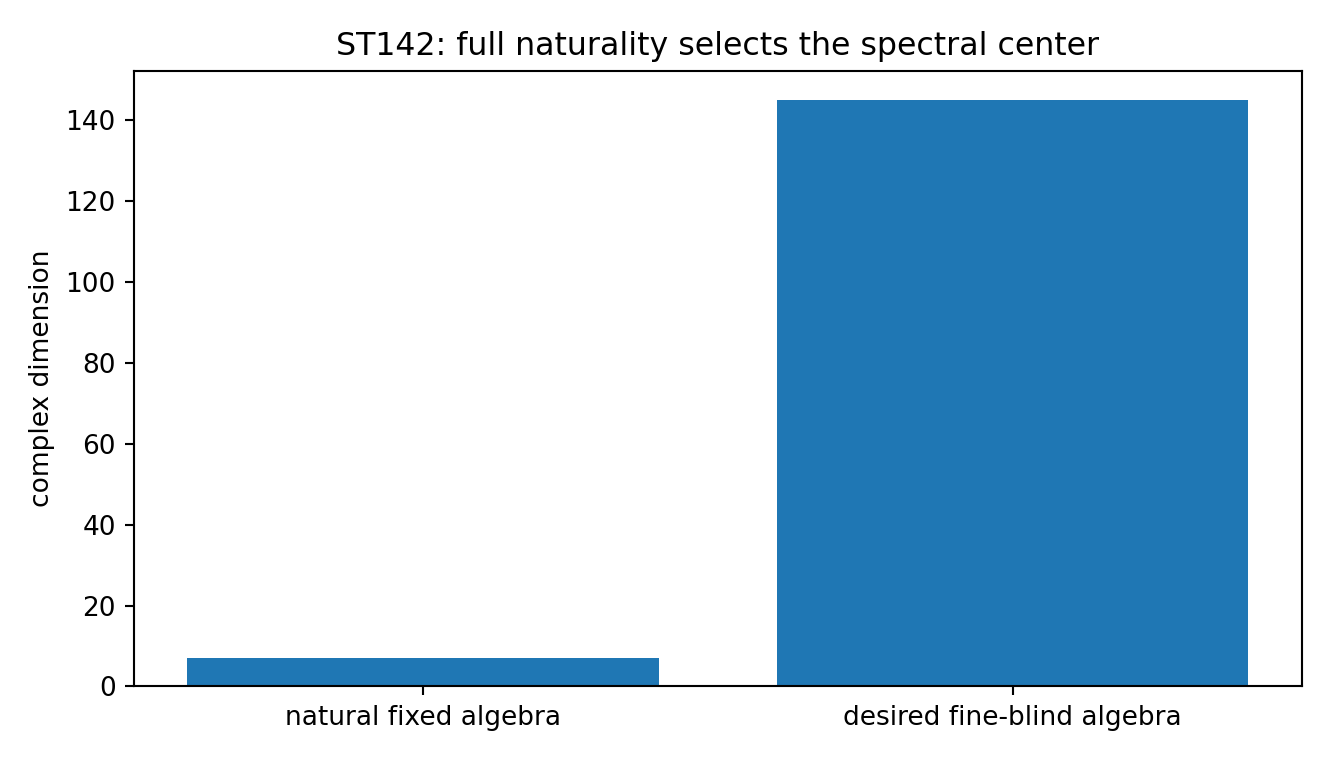
\includegraphics[width=.73\textwidth]{FIN_ST142_ST153_Figures/st142_natural_quotient.png}
\caption{ST142. The full doubled commutant is large, but its conjugation-fixed algebra is only the seven-dimensional spectral center.}
\end{figure}

\statusboundary{} This is not a universal impossibility theorem. A named algebra, region net, preparation family, environment interaction, pointer algebra, instrument, or deliberately reduced automorphism group can evade it. Such an object is additional operational typing, not a consequence of $f(A)$, and QW-2191 remains open.

\section{ST143: complete coordinate-edge star of the lift cone}

At the lift vertex $A$, fix 77 of the 78 coordinate inequalities at their lower endpoints. For each unordered pair $i<j$ the remaining family is
\[
B_{ij}(t)=A+t(E_{ij}+E_{ji}),\qquad 0\le t\le-2A_{ij}=2W_{ij}.
\]

\begin{theorem}[Coordinate-edge star]
Each of the $\binom{12}{2}=66$ off-diagonal families is an exact bounded incident edge. Every point with $t>0$, including the sign-flipped endpoint, is positive definite. The twelve diagonal coordinates give unbounded rays $A+tE_{ii}$, $t\ge0$. These 78 families form the complete coordinate-edge star at $A$.
\end{theorem}

For interior $t$, diagonal dominance is strict in the two changed rows and irreducibility gives positive definiteness. At the endpoint, the associated signed complete graph is unbalanced, so its signed Laplacian has no null vector. The edge counts by cyclic distance are $12,12,12,12,12,6$ for $d=1,\ldots,6$.

\begin{figure}[H]\centering
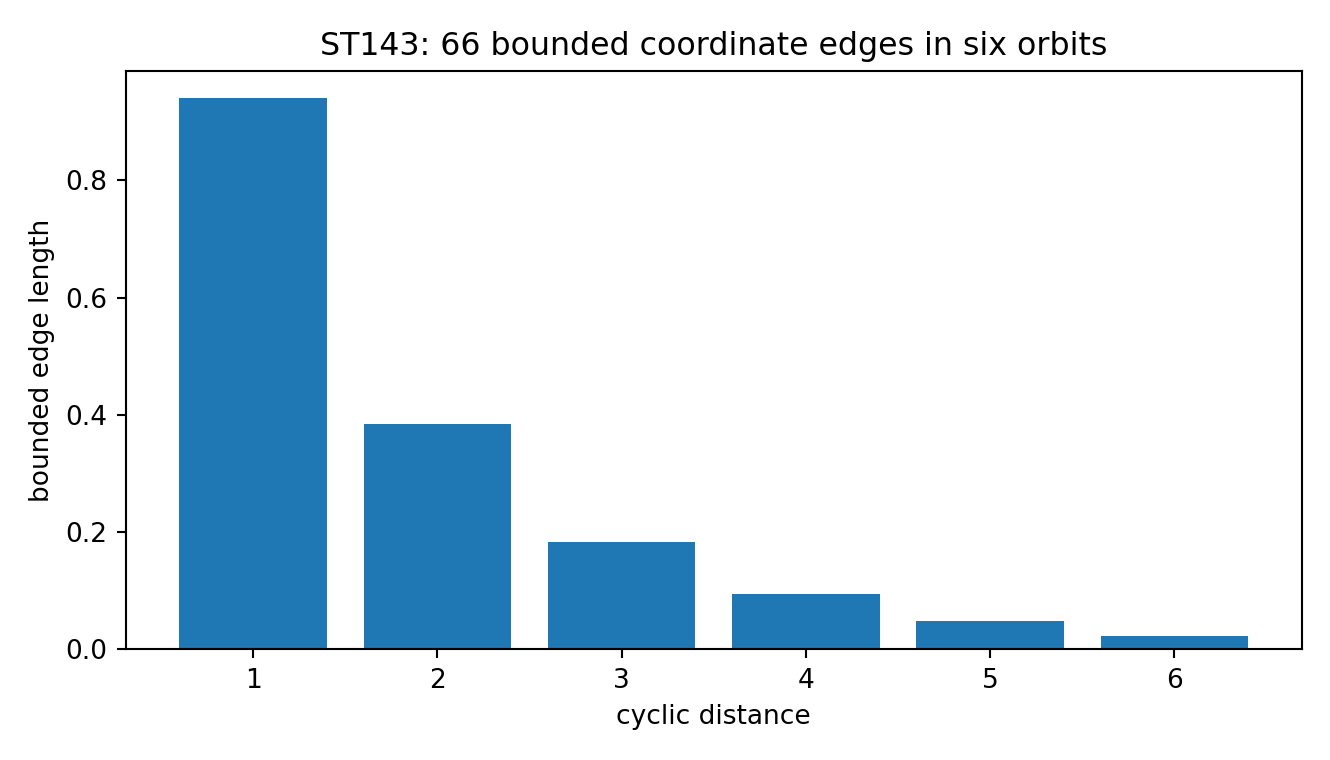
\includegraphics[width=.78\textwidth]{FIN_ST142_ST153_Figures/st143_edge_star.png}
\caption{ST143. Lengths and endpoint minimum eigenvalues for the six cyclic-distance orbits of the 66 bounded coordinate edges.}
\end{figure}

The theorem classifies coordinate incidence only. It does not exclude non-coordinate extreme curves or settle global face adjacency.

\section{ST144: multibasin fold discovery and local interval proof}

The fold system was launched from 64 seeded random starts and five deterministic seeds. Thirty-six runs converged inside the declared filter
\[
-0.3\le\kappa\le0.12,\qquad |q_0|\le3.2,\qquad |q_1|,\ldots,|q_6|\le1.2.
\]
Clustering produced 35 numerical representatives. A local certificate budget was declared in advance for the first 32 representatives. Twenty-nine radius-$10^{-7}$ boxes passed strict outward Krawczyk inclusion; three failed the local test, and three further numerical clusters were not interval-tested.

\begin{theorem}[Certified fold multiplicity]
There exist at least 29 distinct locally unique roots of the declared fold equations. Their certified centers have minimum mutual Euclidean separation
\[
0.3034025048371158,
\]
so their radius-$10^{-7}$ boxes are pairwise disjoint.
\end{theorem}

The familiar positive fold near $\|u\|\approx2.51736$ and $\kappa\approx0.016589$ appears as part of a sign-related family, not as a globally privileged solution.

\begin{figure}[H]\centering
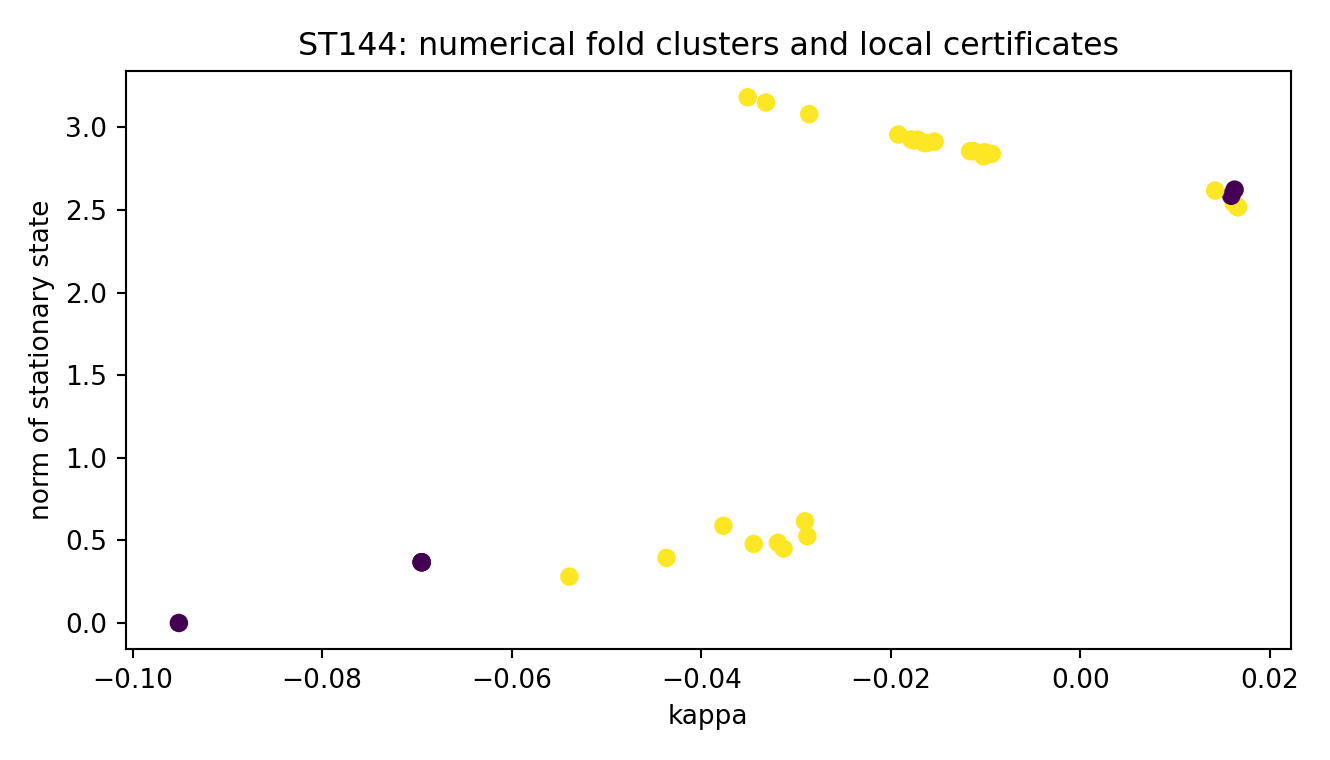
\includegraphics[width=.80\textwidth]{FIN_ST142_ST153_Figures/st144_multibasin.png}
\caption{ST144. Numerical fold clusters in $(\|u\|,\kappa)$ and the subset with accepted local interval certificates.}
\end{figure}

\statusboundary{} The exact statement is ``at least 29 distinct roots.'' The 35-cluster map is strong numerical evidence, not a theorem that exactly 35 roots exist. No interval cover excludes roots between basins or outside the filter.

\section{ST145 and ST146: recovery and constrained selector cost}

\subsection{Coherent balanced-involution leakage}

Let
\[
U=\operatorname{diag}(I_6,-I_6),\qquad \operatorname{Tr}U=0,
\]
and couple a binary syndrome coherently so that pinching produces the orthogonal Choi errors $I$ and $U$ with probabilities $1-p$ and $p=\sin^2\theta$. Let syndrome readout flip $0\to1$ with probability $\delta_0$ and $1\to0$ with probability $\delta_1$. Maximum-likelihood choice of $I$ or $U$ for each observed syndrome is optimal, giving
\begin{equation}
F_e^*=\max\{(1-p)(1-\delta_0),p\delta_1\}
+\max\{(1-p)\delta_0,p(1-\delta_1)\}.
\label{eq:recovery}
\end{equation}
The numerical study uses $\delta_0=0.08$ and $\delta_1=0.17$.

\begin{figure}[H]\centering
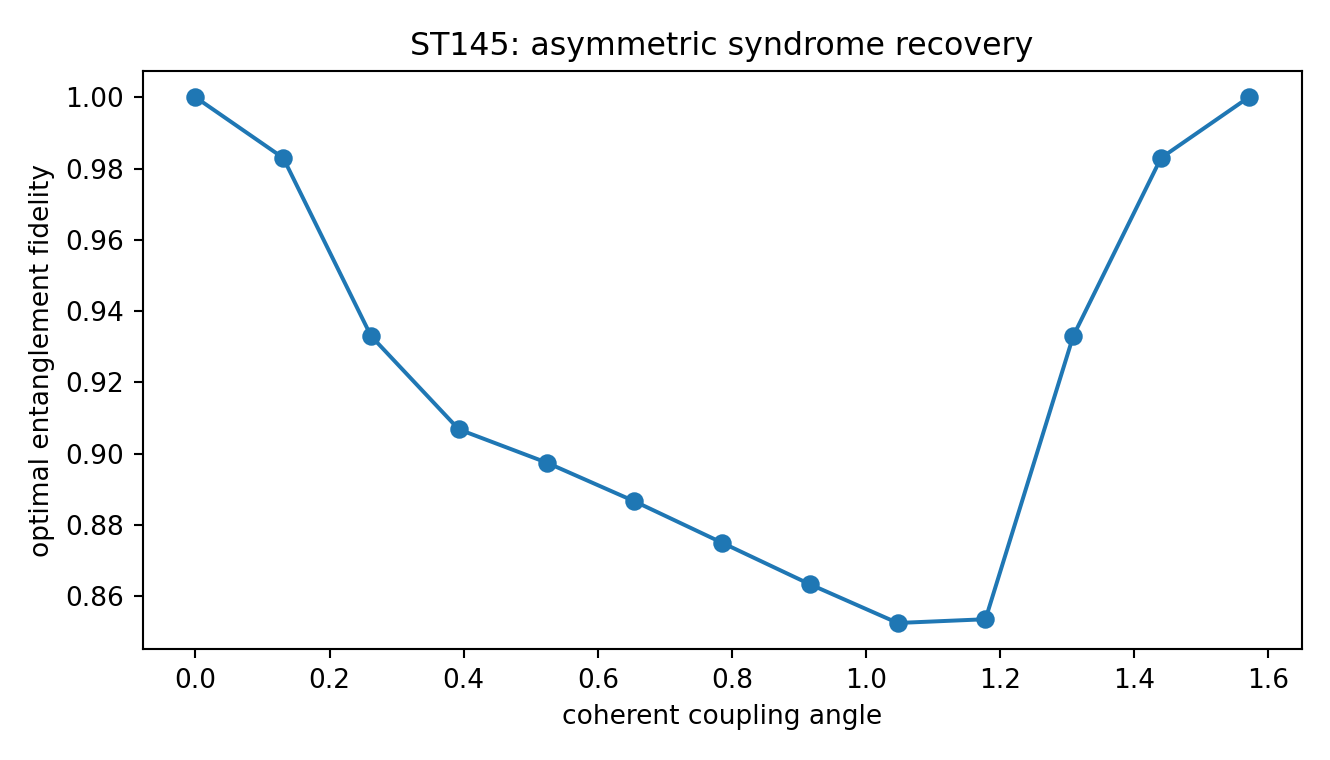
\includegraphics[width=.73\textwidth]{FIN_ST142_ST153_Figures/st145_recovery.png}
\caption{ST145. Exact optimal entanglement fidelity in the declared coherent-syndrome model.}
\end{figure}

\proven{} Equation~\eqref{eq:recovery} is optimal in this model because the two logical errors have orthogonal Choi supports. \statusboundary{} The involution, syndrome coupling, pinching, and readout law are supplied. Generic coherent leakage with a nonbinary unitary spectrum remains open.

\subsection{A positive cost needs a robust operational gap}

Require a vertex measurement distribution to satisfy
\[
p_0-p_j\ge g>0\qquad(j\ne0).
\]
Permutation averaging over the eleven losing outcomes and convexity force the least asymmetric feasible vector to be
\[
p_0=\frac{1+11g}{12},\qquad p_j=\frac{1-g}{12}.
\]
Therefore its minimum total variation from uniform and minimum relative entropy are
\begin{align}
T_{\min}(g)&=\frac{11g}{12},\\
D_{\min}(g)&=\frac{1+11g}{12}\log(1+11g)
+11\frac{1-g}{12}\log(1-g).
\end{align}
Data processing makes these lower bounds valid for any quantum preparation that produces the required distribution.

\begin{figure}[H]\centering
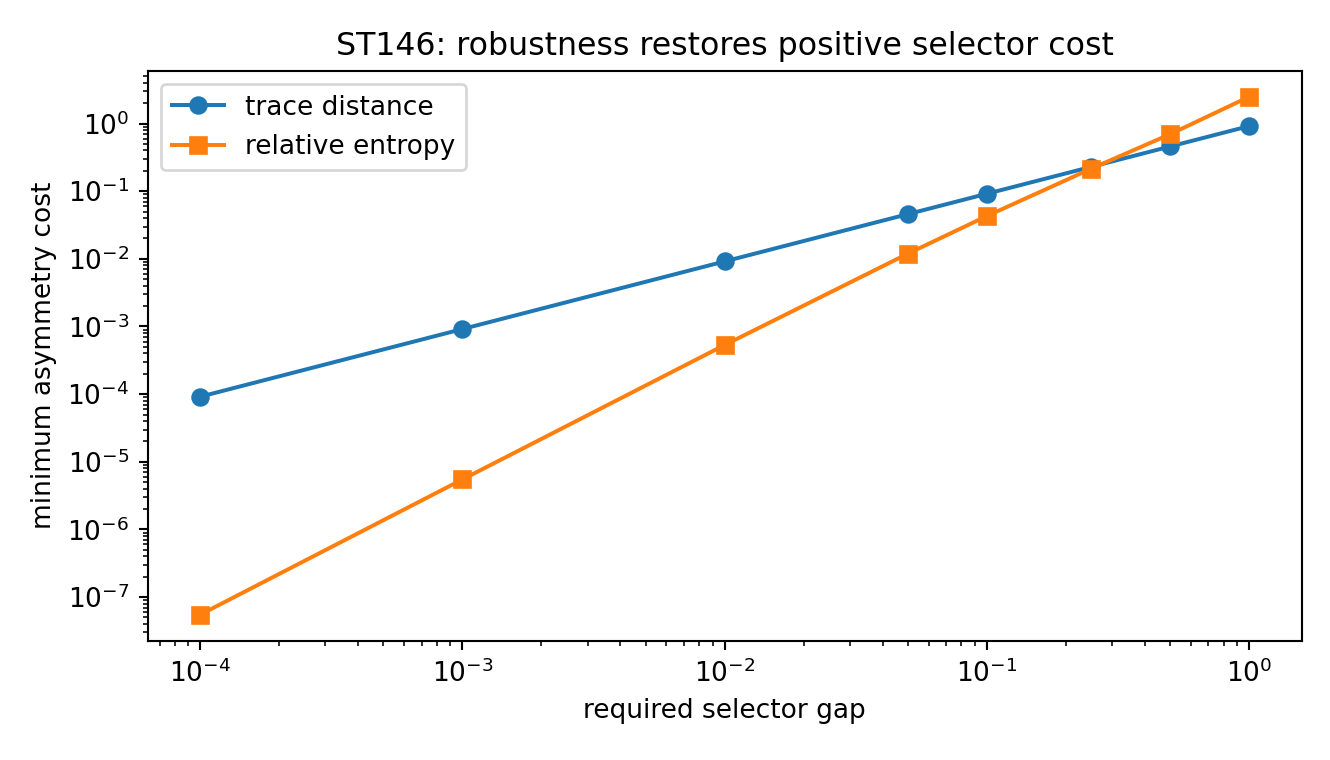
\includegraphics[width=.74\textwidth]{FIN_ST142_ST153_Figures/st146_selector_cost.png}
\caption{ST146. Exact positive selector costs created by the supplied robust probability gap. Both vanish continuously as $g\downarrow0$.}
\end{figure}

\conditional{} This closes the zero-cost loophole of unconstrained selection, but it does not derive $g$, the preferred vertex, or the vertex POVM. Hence it does not discharge the strict selector obstruction.

\section{ST147: symmetric potential, twelve branches, no realized selector}

Consider the bounded $C_{12}$- and reflection-invariant potential
\begin{equation}
V(r,\theta)=-\frac\mu2r^2+\frac\kappa4r^4
-\frac\varepsilon{12}r^{12}\cos(12\theta)+\frac\xi{14}r^{14},
\label{eq:potential}
\end{equation}
with $(\mu,\kappa,\varepsilon,\xi)=(0.2,1,0.05,0.05)$. The associated negative-gradient dynamics provides the stability interpretation.

\begin{theorem}[Twelve-branch equivariant bifurcation]
The nonzero radial stationarity equation has exactly one positive solution in each angular class. There are twelve stable angular branches at
\[
r_+=0.44722791045820004,\qquad \theta=\frac{k\pi}{6},
\]
and twelve angularly unstable branches at
\[
r_-=0.4471921393724437,\qquad \theta=\frac{(2k+1)\pi}{12}.
\]
The twelve minima are symmetry-equivalent.
\end{theorem}

Writing $y=r^2$, the radial polynomial has derivative bounded below by $0.8794367283950617$ on the relevant split domain, proving uniqueness. The angular Hessian alternates in sign.

\begin{figure}[H]\centering
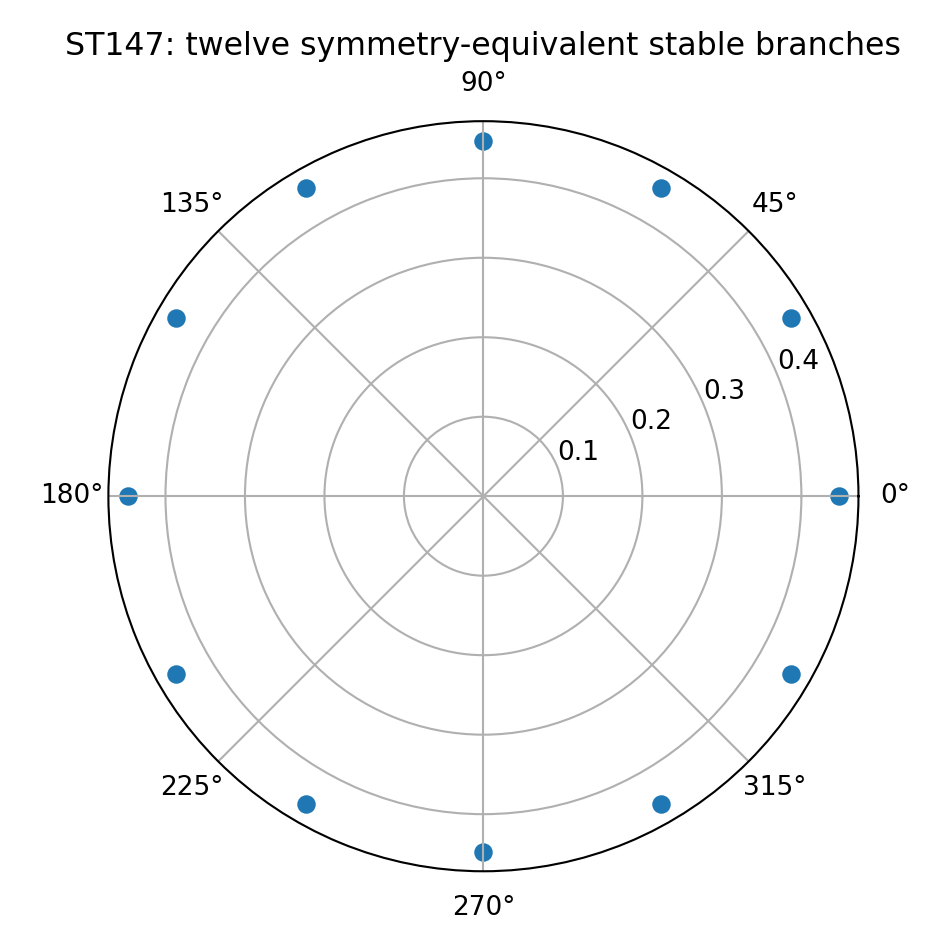
\includegraphics[width=.70\textwidth]{FIN_ST142_ST153_Figures/st147_branches.png}
\caption{ST147. Twelve stable and twelve angularly unstable branches of the constructed equivariant potential.}
\end{figure}

This formalizes symmetry as a reservoir of equivalent possibilities, not as positive feedback by itself. The anisotropic nonlinearity creates amplifiable branches, but an initial condition, fluctuation, boundary condition, or noise history is still required to realize one of them. Moreover $\varepsilon$ and the other coefficients have not been derived from the strict operator.

\section{ST148: certified nuisance continuation and method boundary}

The ST136 stationary Chernoff root was continued over common symmetric halfwidth boxes in $(q_0,q_1,\delta)$. For each halfwidth the proof searches enlarged boxes in the stationary variables and accepts only strict Krawczyk inclusion for the entire nuisance box.

Ten bisection steps give
\[
h_{\rm pass}=1.4599609375\times10^{-5},\qquad
h_{\rm fail}=1.4609375\times10^{-5},
\]
with bracket width $9.765625\times10^{-9}$.

\begin{figure}[H]\centering
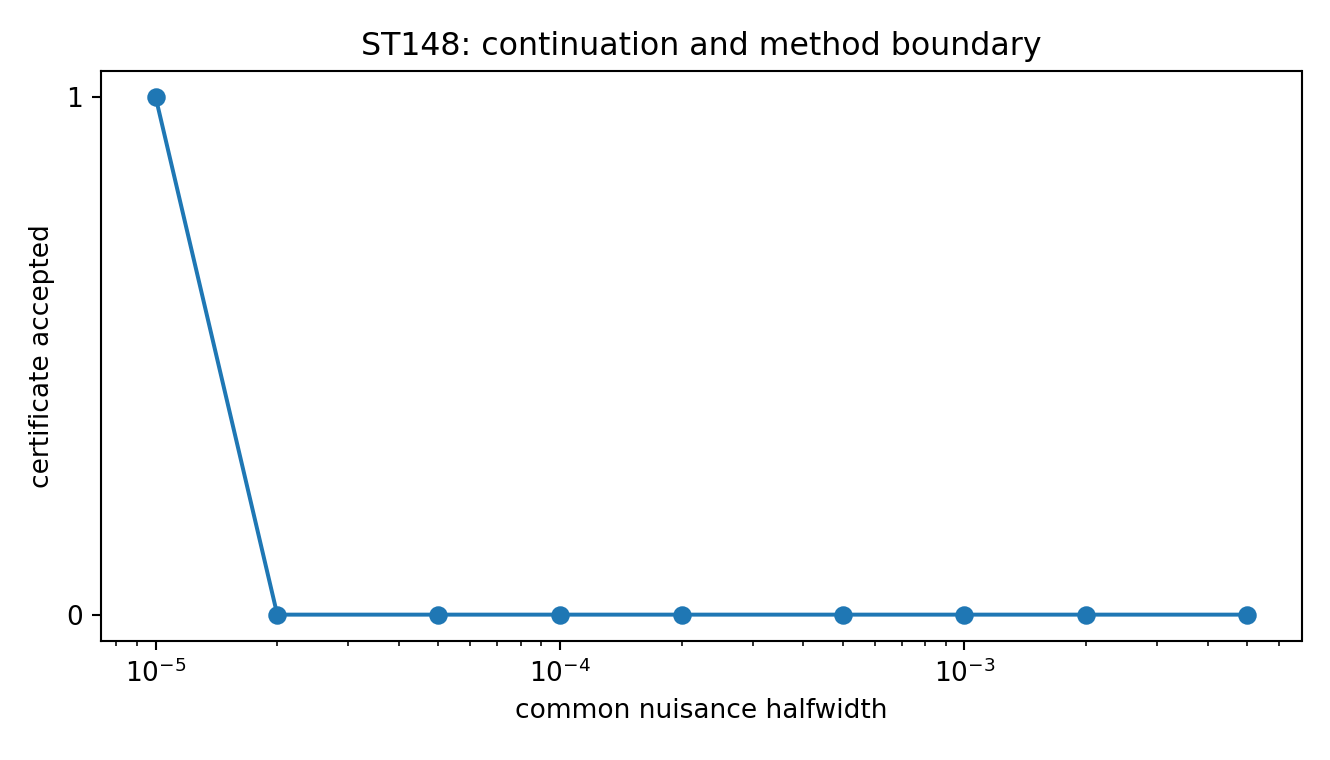
\includegraphics[width=.78\textwidth]{FIN_ST142_ST153_Figures/st148_continuation.png}
\caption{ST148. Passed and failed common nuisance halfwidths. The boundary belongs to the declared box-and-preconditioner certification method.}
\end{figure}

\proven{} Every nuisance triple in the largest passed box has exactly one stationary root in its common certified root box. \statusboundary{} Failure at the next halfwidth is not evidence that the root disappears, that a physical transition occurs, or that a global Chernoff optimum changes. Adaptive interval subdivision is needed before interpreting the boundary geometrically.

\section{ST149 and ST150: refinement cohomology and typed causal nets}

\subsection{Executable affine cohomology on a finite DAG}

For each source-to-node path, propagate an affine bit map $x\mapsto ax+b$, with $a\in\mathbb F_2$ and $b$ a linear form in edge-twist bits. Unequal $a$ values give an immediate parity obstruction. If all $a$ values agree, path independence is equivalent to a finite XOR system. Gaussian elimination determines its rank $r$ and hence $2^{E-r}$ coherent twist assignments.

\begin{theorem}[Finite refinement criterion]
The path-transport algorithm is necessary and sufficient for coherence of every finite topologically ordered affine refinement DAG.
\end{theorem}

For the six-node, eight-edge all-odd example, the XOR rank is three and there are $2^{8-3}=32$ coherent twist assignments. Changing one degree creates parity obstructions at nodes 3 and 5 and makes the coherent count zero. This is an exact finite certificate, but the graph, degrees, and twists remain supplied.

\subsection{When a causal net selects an algebra}

Let
\[
\mathcal A(\{1\})=M_2\otimes I,qquad
\mathcal A(\{2\})=I\otimes M_2,qquad
\mathcal A(\{1,2\})=M_4,
\]
with labeled singleton regions. Each factor is the commutant of the other, and the normalized-trace conditional expectation onto each factor is unique.

\begin{proposition}[Sufficiency and deletion boundary]
The labeled atomic net selects the two conditioning algebras. Removing the singleton labels leaves a swap ambiguity. Removing the factor algebras while retaining only trace/product independence restores the continuum of conjugate choices exhibited in ST138.
\end{proposition}

Thus an operational causal net can solve the algebra-selection problem, but only because region labels and local algebras are part of the input. It does not derive their physical interpretation from $A$.

\section{ST151: Markov-modulated finite-count discrimination}

Let detector availability follow the stationary Markov chain
\[
P=\begin{pmatrix}0.9&0.1\\0.2&0.8\end{pmatrix},
\qquad \pi=\left(\frac23,\frac13\right),
\]
where the first state is bad and emits an erasure, while the good state emits a Bernoulli observation with $p_0=0.72$ or $p_1=0.94$. The Dobrushin contraction coefficient is $0.7$.

Conditional on $K$ good events, the exact Bayes error is the $K$-sample binomial overlap. Averaging over the exact Markov distribution of $K$ gives the finite-$n$ law. The tilted two-by-two transfer matrix has spectral radius
\[
\rho_*=0.9851012493279235<1,
\]
and therefore exponent
\[
-\log\rho_*=0.015010851896839685.
\]

\begin{figure}[H]\centering
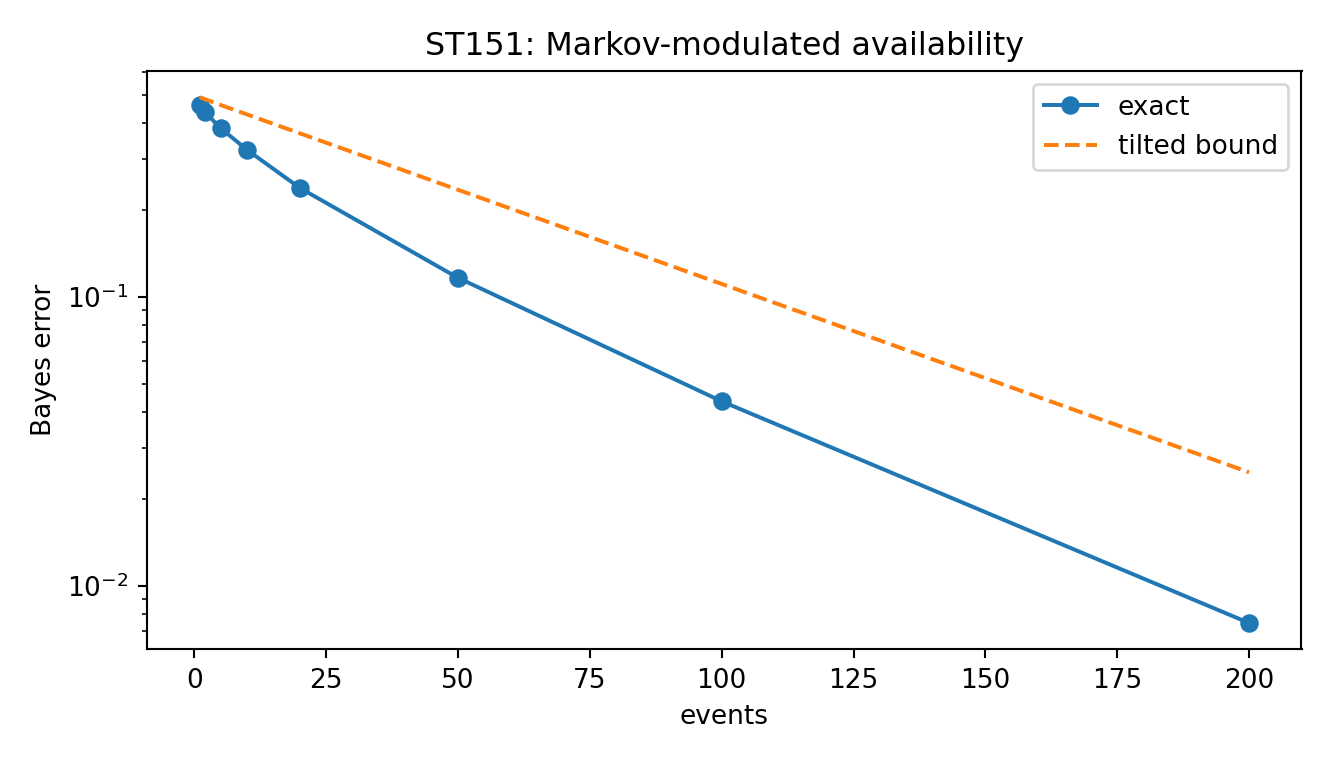
\includegraphics[width=.75\textwidth]{FIN_ST142_ST153_Figures/st151_markov_counts.png}
\caption{ST151. Exact Bayes error and valid Chernoff upper bound under Markov-modulated availability.}
\end{figure}

The exact Bayes error falls from $0.4633333$ at $n=1$ to $0.00744291$ at $n=200$. The theorem is conditional on the transition matrix, stationary law, emissions, and observable erasure. A fully hidden non-erasure HMM remains untested.

\section{ST152: sharp bath dimension for global Gibbs reset}

Treat the twelve eigenvalues of $A$ as a dimensionless Hamiltonian and set $\gamma=e^{-\beta A}/\operatorname{Tr}(e^{-\beta A})$ with the supplied $\beta=0.8$. The exact replacement channel is
\[
\mathcal R_\gamma(\rho)=\gamma\operatorname{Tr}\rho.
\]

\begin{theorem}[Exact bath-dimension minimum]
Any unitary implementation of $\mathcal R_\gamma$ using a bath of dimension $m$ and an initial bath state of rank at most $m$ satisfies $m\ge12$. Equality is attained by a twelve-level bath with $H_B=A$, state $\gamma$, and full SWAP, which commutes with $A\otimes I+I\otimes A$.
\end{theorem}

\textit{Proof.} A full-rank replacement channel on dimension $d$ has Choi rank $d^2$. A unitary dilation with bath dimension and initial rank at most $m$ has Kraus rank at most $m^2$. Hence $m^2\ge d^2$, so $m\ge d=12$. The isospectral SWAP construction attains the bound. \hfill$\square$

For $m<12$, the normalized Choi-state trace distance on a maximally entangled input is bounded below by the spectral tail beyond the largest $m^2$ eigenvalues of $I/12\otimes\gamma$. Selected bounds are $0.914367$ at $m=2$, $0.462052$ at $m=6$, $0.150613$ at $m=10$, and $0.0768878$ at $m=11$.

\begin{figure}[H]\centering
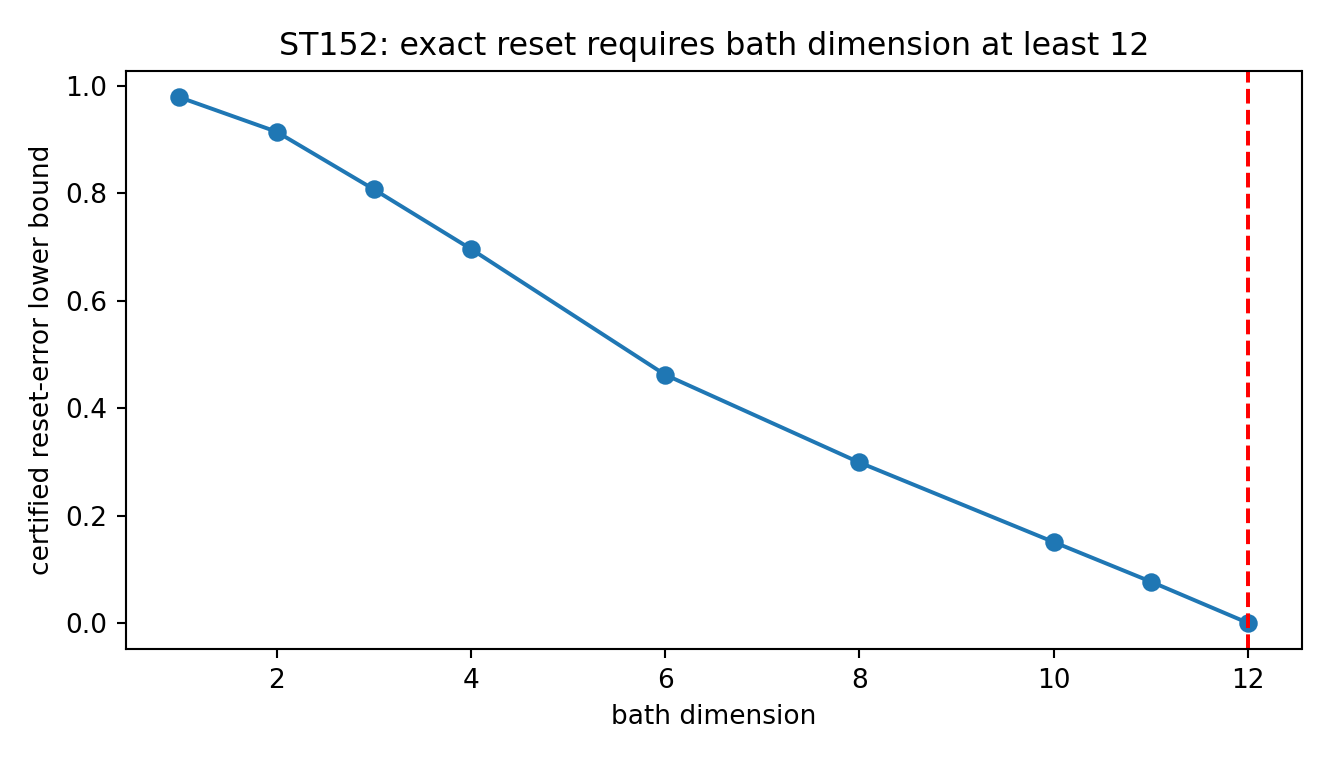
\includegraphics[width=.73\textwidth]{FIN_ST142_ST153_Figures/st152_bath_bound.png}
\caption{ST152. Rigorous entangled-input approximation lower bounds versus bath dimension. Exact reset first becomes possible at $m=12$.}
\end{figure}

\statusboundary{} This is a resource theorem, not a derivation of thermodynamics from the strict kernel. The Hamiltonian interpretation, inverse temperature, bath preparation, SWAP time, energy scale, and apparatus are supplied.

\section{ST153: complete minimax detector classification}

For the declared entrywise-nonnegative, positive semidefinite, unit-trace adversary class, the minimax value from ST141 is $1/12$. ST153 determines all detectors attaining it.

\begin{theorem}[Complete optimizer set]
A detector $H$ is minimax optimal if and only if
\[
H\succeq0,\qquad \operatorname{Tr}H=1,\qquad
H_{ii}=\frac1{12},\qquad H_{ij}\ge0\quad(i\ne j).
\]
The depolarizing detector map $H\mapsto(1-\delta)H+\delta I/12$ preserves this complete set.
\end{theorem}

The adversarial matrices $E_{ii}$ force a uniform diagonal. If $H_{ij}<0$, a normalized rank-one adversary built from $e_i+\epsilon e_j$ lowers the response below $1/12$. Conversely every nonnegative off-diagonal pairs nonnegatively with the adversary cone. The continuum
\[
H_c=\frac{(1-c)I+cJ}{12},\qquad 0\le c\le1,
\]
contains optimal points of rank twelve down to rank one. Thus noise robustness does not imply uniqueness.

\section{What the batch changes in the interpretation of FIN}

The results sharpen five structural conclusions.

\begin{enumerate}
\item \textbf{Information cannot mean spectrum alone.} Full naturality with respect to the strict doubled dynamics retains only seven spectral labels. Geometry, operational sectors, instruments, orientation, and records are not recovered.
\item \textbf{Symmetry is a space of possibilities, not a selector.} The $C_{12}$ potential rigorously creates twelve stable alternatives. It does not choose the actual alternative. Positive feedback begins only after a branch perturbation and a dynamical gain are specified.
\item \textbf{Medium-independent information needs an operational invariant.} ST149 and ST150 show two components of such a notion: path-independent transport and typed local algebras. Neither is derived from $A$ alone. A physical carrier can change while an abstract operational equivalence persists only after encodings, instruments, and comparison maps are defined.
\item \textbf{Projection is many-to-one and therefore resource-bearing.} Quotients, pinching, syndrome readout, erasure flags, and Gibbs reset all require a declared map or environment. The existence of mathematical reductions is compatible with a projection interpretation, but does not prove that the observed universe is a projection of FIN.
\item \textbf{Thermal physics needs more than a spectral state.} Even after choosing $A$ as a Hamiltonian and $\beta$, exact preparation of the full Gibbs state has a sharp environmental cost. The strict dimensionless spectrum still supplies neither joules nor seconds.
\end{enumerate}

The scale obstruction remains channel-specific. Unitary and heat channels use rates proportional to eigenvalues of $A$, whereas the wave channel $\cos(t\sqrt A)$ uses frequencies proportional to $\sqrt\lambda$. Under $A\mapsto cA$, unitary phase time rescales as $t\mapsto t/c$, while wave time rescales as $t\mapsto t/\sqrt c$. Solitonic frequency therefore supplies dimensionless phase relations, not a calibrated physical second.

\section{Recommended programs ST154--ST165}

\begin{longtable}{@{}p{0.07\textwidth}p{0.10\textwidth}p{0.73\textwidth}@{}}
\toprule ID & Priority & Bounded research target\\\midrule\endfirsthead
\toprule ID & Priority & Bounded research target\\\midrule\endhead
ST154 & 1 & Classify environment-induced superselection quotients with a typed interaction but without a predeclared fine algebra.\\
ST155 & 2 & Interval-cover the reduced fold domain around every ST144 cluster and certify exclusion boxes; separate root count from basin sampling.\\
ST156 & 3 & Derive coherent-leakage recovery for a general unitary spectrum rather than a balanced involution.\\
ST157 & 4 & Derive selector-cost bounds from action, energy, or finite-time preparation budgets instead of an imposed probability gap alone.\\
ST158 & 5 & Couple the $C_{12}$ anisotropy coefficient to a strict-derived state, or prove a source obstruction in a declared class.\\
ST159 & 6 & Replace the single-box ST148 continuation by adaptive interval subdivision and distinguish a genuine root boundary from preconditioner failure.\\
ST160 & 7 & Classify refinement-DAG affine cohomology under composition and coarse-graining functors.\\
ST161 & 8 & Test whether a labeled atomic causal net can be reconstructed from a supplied instrument-tomography table.\\
ST162 & 9 & Remove the observable erasure flag from ST151 and certify a genuinely hidden HMM exponent.\\
ST163 & 10 & Bound approximate-reset bath resources under locality, bounded interaction strength, and finite time.\\
ST164 & 11 & Classify extreme points, exposed faces, and affine dimension of the complete ST153 optimizer spectrahedron.\\
ST165 & 12 & Integrate gauge, preparations, clock, bath, apparatus, instruments, environment, and independent record into one minimal operational tuple; then repeat axiom deletion.\\
\bottomrule
\end{longtable}

The highest scientific priority is ST154 because it attacks the gap between a bare spectral operator and a physically meaningful observable algebra without naming the answer in advance. ST155 is the strongest local proof opportunity. ST165 is the synthesis program, but it should follow the resource classifications rather than silently assume them.

\section{Reproducibility and audit trail}

The executable source is \texttt{fin\_st142\_st153\_research.py}. It writes one master JSON file, one CSV outcome table, eight specialized JSON certificates, and nine figures. The deterministic seed is \texttt{20260823}. The recorded environment is Python 3.12.3, NumPy 1.26.4, and SciPy 1.17.1.

The test suite \texttt{test\_fin\_st142\_st153.py} contains 33 checks. Live tests cover the strict spectrum, doubled-algebra dimensions, lift-edge endpoints, a Krawczyk certificate, recovery formulas, constrained selector bounds, branch radii, nuisance boxes, DAG consistency, causal-net identities, Markov error bounds, bath-rank limits, and minimax necessity/sufficiency examples. Frozen JSON checks are supplemented by live function evaluations.

Specialized machine-readable packets are supplied for ST143, ST144, ST145, ST148, ST149, ST151, ST152, and ST153. File integrity is recorded separately in \texttt{FIN\_ST142\_ST153\_SHA256SUMS.txt}.

\section{Final verdict}

\resultbox{\textbf{Deepest surviving interpretation.} FIN presently supports a finite spectral-information core together with a growing family of rigorously classified operational completions. The strict operator determines common spectral channels and strong symmetry constraints. It does not, by itself, determine the fine observable algebra, a realized selector branch, dimensional time or energy, a bath, preparation, instrument, apparatus, or record. The new theorems make this separation sharper: naturality collapses to the spectral center; constrained resources create positive selection cost; typed nets restore algebraic meaning; and full thermal reset has a sharp environmental dimension.}

The batch supplies no strict fine-gauge source, QW-2191 discharge, strict source of anisotropy, canonical dimensional scale, calibrated clock, laboratory apparatus or record, legacy-to-strict completion, legacy physical-role transfer, Standard Model, gravity, total physical Lagrangian, physical projection theorem, or Theory-of-Everything closure. These absences are not rhetorical qualifications; they are the current mathematical frontier.

\end{document}
